\chapter{Gestion de version de code source}

\section{Git : le gestionnaire de version}

Les logiciels de gestion de versions ou VCS\, \footnote{\emph{Version Control
System.}} sont utilisés principalement par les développeurs. En effet, ils sont
quasi exclusivement utilisés pour gérer des codes sources, car ils sont
capables de suivre l’évolution d’un fichier texte \emph{ligne de code par ligne de
code.} Ces logiciels sont fortement conseillés pour gérer un projet
informatique.

Ils retiennent qui a effectué chaque modification de chaque fichier et
pourquoi. Ils sont par conséquent capables de dire qui a écrit chaque ligne de
chaque fichier et dans quel but ; si deux personnes travaillent simultanément
sur un même fichier, ils sont capables d’assembler (de fusionner) leurs
modifications et d’éviter que le travail d’une de ces personnes ne soit écrasé.

Ces logiciels ont donc par conséquent deux utilités principales :
\begin{itemize}
    \item suivre l’évolution d’un code source, pour retenir les modifications
effectuées sur chaque fichier et être ainsi capable de revenir en arrière en
cas de problème ;
    \item travailler à plusieurs, sans risquer de se marcher sur les pieds.
Si deux personnes modifient un même fichier en même temps, leurs modifications
doivent pouvoir être fusionnées sans perte d’information.
\end{itemize}

\subsection{Les rudiments}

\emph{Un commit} correspond à un enregistrement des modifications dans le
temps.  Admettons un fichier contenant un paragraphe, si nous ajoutons un
deuxième paragraphe, le fichier sera considérer comme modifié par Git\,
\footnote{Créé par Linus Torvalds, qui est entre autres l’homme à l’origine de
Linux. Il est de type distribué.}, pour enregistrer la modification on effectue
un commit.  L'analogie la plus simple est celle des jeux vidéos ou vous
sauvegardez votre progression à chaque étape franchie.

\emph{Une branche} représente une \og copie virtuelle \fg{} du dossier contenant
les fichiers sources. En effet, il est possible à partir d'un dépôt de le
cloner virtuellement et de basculer de l'un à l'autre pour par exemple
développer sur la branche principale les nouvelles fonctionnalitées et sur
l'autre branche les corrections de bug.

\begin{center}
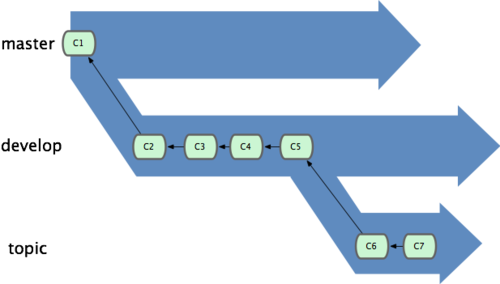
\includegraphics{images/branches.png}
\end{center}

\emph{La fusion} est l'opération de rassemblement des deux branches en une,
c'est-à-dire dans le cas précédent de regrouper les corrections de bug avec les
nouvelles fonctionnalitées.

Les fondamentaux ayant été acquis, j'ai trouvé plusieurs solutions à la
problématique principale qui est la suivante :\\ \quote{Peut-on fusionner des
branches tout en choisissant de ne pas fusionner tout les commits ?}\\

\begin{itemize}
    \item Tout dabord la commande \emph{git chery-pick \og nomducommit \fg{}}
        permet de \og cueillir \fg{} le commit que l'on veut fusionner.
    \item Ensuite on peut aussi rassembler les deux branches puis faire un
        \emph{git revert \og nomducommit \fg{}} pour retirer le commit après la
        fusion.
    \item Enfin faire trois branches distinctes pour ne pas avoir à faire les
        opérations ci-dessus.
\end{itemize}

Git répondant au besoin de l'entreprise, il a fallut que j'effectue des
recherches pour que la migration Subversion\, \footnote{Le logiciel de gestion
de versions le plus utilisé à l’heure actuelle. Il est de type centralisé.}
vers Git ce fasse sans perte.

\subsection{L'installation} % (fold)
\label{sec:L'installation}

A peu près au milieu du stage, nous nous sommes heurté a un problème technique.
Le serveur de l'entreprise ne contenai pas de version réçente de Git. En
sachant que celui-ci est mutualisé\, \footnote{L'hébergement mutualisé est un
concept d'hébergement internet destiné principalement à des sites web, dans un
environnement technique dont la caractéristique principale est d'être partagé
par plusieurs utilisateurs. L'administration du ou des serveurs est assurée par
un intervenant tiers tel qu'OVH.}, nous n'avions pas les autorisations
nécessaire pour installer une nouvelle version.

Les logiciels libres sont réputé pour être rétro-compatibles mais en toute
logique il ne dispose pas des nouveautés sans les mettre à jour. Le problème ce
situe sur le fait de pouvoir modifier des branches distantes dites "de suivi".
Cette fonctionnalité permet à plusieurs développeurs de travailler en même
temps sur une branche différente de celle par defaut, par exemple pour
experimenter de nouvelles implémentation à plusieurs. A ce moment là j'ai été
très déçu et pensais mon travail inutilisable. Cependant, mes éfforts n'ont pas
été vain puisque M.Dubourg après des recherches à trouver sur internet un
utilisateur ayant reussi à installer git sur un serveur mutualisé. Nous
n'avions peut-être pas les droits d'accès au dossiers des programmes mais rien
ne nous empechai de compiler git a partir des sources pour nous crée en locale
le logiciel\, \footnote{Le problème ne ce serai pas posé si j'avais lu le
chapitre traitant de la compilation dans mon livre Linux, j'ai découvert cette
méthode qu'après le stage...}. Ceci étant fait, en redéfinissant la variable
système qui stocke les chemins des applications, nous avons pu utilisées notre
compilé dernier cri.
% section L'installation (end)

\subsection{Le passage fatidique} % (fold)
\label{sec:Le passage fatidique}

Trois jours avant mon départ, le grand déménagement s'impose. Toute la partie
étude et confection du tutoriel git prend forme car j'ai basculer tout les
projets qui était au préalable sur Subversion vers Git tout en gardant
l'historique des changement provenant de SVN. Après quelques recherche, une
commande de Git ma permis de répondre à ce besoin.
% section Le passage fatidique (end)

\section{Les utilitaires} % (fold)

Nous avons longuement discuté sur le côté technique de git. En effet cette
outil est à la base un logiciel libre provenant de linux et n'as pas
d'interface graphique, ce choix est établi sur le fait qu'un développeur n'as
pas forcement besoin de ça pour travailler (Sans nul doute que pour un
graphiste, une souris est un élément indispensable pour ses créations mais pas
pour produire du code) et aussi que cette outil regorge de fonctionnalité et
donc très difficile à simplifier à travers une interface ne pouvant fonctionner
qu'avec une souris. L'équipe n'étant pas très féru de ligne de commande et le
logiciel TortoiseGit reprenant que les fonctions éssentielle de Git, il a fallu
que je conçois des petits programmes qui fonctionne en un clic pour simplifier
les choses répétitives.

% section Introduction (end)

\subsection{Lister les dépôts du serveur}

Mon travail suivant consistait a lister les dépôt Git dans une page php. En
effet, le fait que le serveur OVH centralise les codes sources de la société,
les developpeurs devait récuperer une copie de ses dossiers pour pouvoir
travailler dessus, le problème étant qu'il devait lancer FilleZilla pour
connaitre les noms des dossiers Git puis recopier la bonne url avec le bon nom
est très fastidieux. J'ai donc à l'aide de mes connaissance en système UNIX
crée un script en langage PHP qui analyse un dossier défini et qui liste les
differents dépôt tout en leur métant les bonnes addresses de téléchargement en
préfixe. Du coup, un simple copier-collé du lien du dépôt voulu dans
tortoiseGit suffit à cloner. Gain de productivité et de simplicité en somme.

\subsection{Mise à jour locale automatique} % (fold)

Les developpeurs possédent des clones des dépôts distants\, \footnote{Ils ce
trouvent tous sur le serveur OVH qui sert de point de rencontre comme nous
l'avons vu.} en locale pour bien évidament pour maintenir le code source. Le
fait qu'il y ai une multitude de dépôts implique qu'il faut mettre à jour les
clones locaux à chaque fois pour récuperer les modifications des autres
développeurs ce qui est très répétitif et fastidieux. J'ai donc crée un script
Batch\, \footnote{Désigne un fichier contenant une suite de commandes qui
seront traitées automatiquement par Windows \copyright.} qui parcours tout les
dossiers contenant les sources des dépôts et les mets a jour. Pour cela j'ai
parcouru la documentation de la console windows et ça n'as pas été évident du
tout. Pour l'anecdote, je devais à partir de mon MacBook\, \footnote{Système de
type UNIX.}, lancer une machine virtuelle windows\, \footnote{À partir du
logiciel VirtualBox.} pour crée mon script batch qui lance une console Linux
pour faire la mise à jour...

% section Mise à jour distante automatique (end)

\subsection{Mise en production automatique} % (fold)

Une fois que les développeurs sont satisfait de leurs modifications, il doivent
mettre à jour le dépots distant pour partager leurs travaux. Une fois ses
modifications validées par le chef de projet, celui-ci doit mettre en ligne sur
le dépôt de production. J'ai crée un script Batch pour que ça ce fasse en un
clic.

% section Mise en production automatique (end)
\clearpage
